\chapter{Ranking Context Networks}

So far, our treatment of context networks had made an assumption: context solely consists of events co-occurring with the photo-capture events, and these events are obtained from data sources. The second part of the assumption is not always true in practice. For example, a person's roommate might be a last minute addition to a road trip, who was neither on the email chain or the facebook event, will be ranked very low by the discovery algorithm. A professor whose students are receiving best paper award but was not part of the author list herself might be present at the award ceremony because the conference is being hosted 50 kilometers from her university. Similarly, people at a concert might run into acquaintances because they share the same musical interests. In these cases, the data sources will provide incomplete contextual information which leads the discovery algorithm to rank some candidates poorly.

In this chapter, we will attempt to address this problem of boosting the performance of the CueNet framework by introducing a technique to rank candidates based on their participation profile in previous context networks, personal interests or information. We will present our intuition through a series of examples, and introduce a technique similar to PageRank, which is used to rank pages on the world wide web. In our case, we will rank people in the \texttt{CandidateSet} given set of context networks. Our main differences will lie in the initialization of the score matrix and the propagation of scores \textit{across} the different context networks.

\section{Intuition}

\begin{figure}[t]
\centering
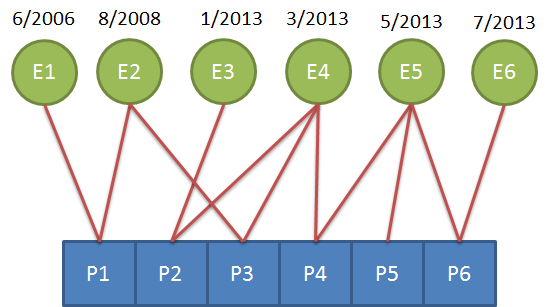
\includegraphics[width=0.65\textwidth]{media/chapter6/intuition-time-example.png}
\caption{Propagating values through temporal relations.}
\label{fig:time-example}
\end{figure}

Consider the very simple context networks shown in figure \ref{fig:time-example}. Each network contains an event, and they have a set of participants. Lets assume that all events \texttt{E1} - \texttt{E6} are of the same type, and occurred at the same location. But as shown in the figure the time of occurrence varies. Lets say that the hit ratio for tagging \texttt{E1} - \texttt{E5} is 100\%. But \texttt{E6} has a few untagged faces, and no more data source is able to provide additional context. The context discovery algorithm has a basic ranking algorithm which looks all social networks (temporal or not), and ranks entities based on whether they have any relations with its participants (in this case, \texttt{P6}). In this case, we could find that \texttt{P6} has participated with \texttt{P5} and \texttt{P4} in event \texttt{E5}. The voting algorithm stops if \texttt{P5} and \texttt{P4} are not found in the \texttt{E6}'s photo. But looking at all the networks, it makes sense to say that since these are all events of the same type, we could say that \texttt{P2}, \texttt{P3} and \texttt{P4} have participated in this same event a few months before \texttt{E6}'s occurrence, and therefore it is possible that \texttt{P2} and \texttt{P3} also participating in \texttt{E6}. With the same idea, we can also \texttt{P2} and \texttt{P1} participated in the same event many years, and therefore is a very low but non-zero chance that \texttt{P1} is present in the photo.

Similarly, look at figure \ref{fig:location-example} where the context networks are exactly as before, but the types of events now vary. We show the type of the event above the event nodes. Their timestamps and location properties are exactly as before. Here, can we exploit some ontological properties about event similarities to propagate scores. If we know that \texttt{L1} is a \texttt{conference}, \texttt{L2} is a \texttt{music-event} and \texttt{L3} is a party, then can we say that \texttt{L2} events are more likely to contain the untagged person than the \texttt{conference} events. 

\begin{figure}[h]
\centering
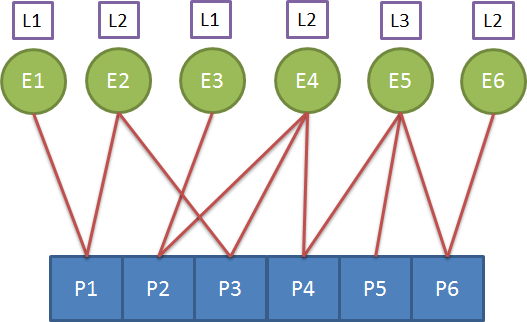
\includegraphics[width=0.65\textwidth]{media/chapter6/intuition-location-example.png}
\caption{Propagating values through ontological event relations.}
\label{fig:location-example}
\end{figure}

Similarly, we can use social and spatial relationships to propagate rank scores to more individuals than just making a single hop as in the context discovery algorithm to reach a wider set of candidates.

\subsection{Rank Propagation}

The rank propagation technique is used to rank nodes in a directed graph. Most commonly seen versions are the HITS algorithm invented by Jon Kleinberg \cite{kleinberg1999authoritative} and the PageRank algorithm developed by Larry Page and Sergey Brin \cite{page1999pagerank}. The idea in the latter is to assign a set of initial values to a subset of nodes, and propagate a fraction of these values to their neighbors. Each iteration of the algorithm propagates their scores to the neighboring nodes until the overall ordering of the nodes, according to their scores, does not change. In practice, a few iterations ($\leq$ 10) on web scale graphs is sufficient.

In this chapter, we will modify the rank propagation technique to rank entities on a given set of context networks, to determine who might be participating in a new events. We will initialize scores of the nodes on the basis of what is known about the new event -- its type, the participating entities, and propagate the scores based on a set of propagation functions which we will introduce later. Since the basic propagation algorithm is an expensive one, we will look at some ways to reduce the size of the context networks, so the algorithm converges quickly, and still provides useful results.

\section{Preliminaries}

Let us first take a look at how rank propagation works in simple directed graphs. The Pagerank \cite{page1999pagerank} algorithm, designed to rank large web graphs is an extension of this idea. The intuition behind Pagerank is known as the random surfer model. The rank propagation models the behavior of a random web surfer who follows a few links and then gets bored and jumps to a random part of the web graph. The final scores of the ranking algorithm converge to the probabilities of such a surfer sees a particular page, while traversing the web in this fashion. Consider the graph in figure \ref{fig:pr-graph-example} \footnote{This example is adapted from Wikipedia (http://en.wikipedia.org/wiki/PageRank)}. Let the initial scores of all nodes be 0.25. In the first iteration of the algorithm, the score of node A would be computed as follows. Since A has three incoming edges from nodes B, C and D, each of these nodes would transfer a portion of their score to A. Since B has two outgoing edges, it transfers half of it scores through each of them, C transfers all of its score to A and D transfers one-third of its score to A. At the completion of this iteration, page A has a score of $PR(B)/2 + PR(C) + PR(D)/3 = 0.458$. In this fashion, the scores for all the nodes are computed in each iteration, until the scores converge.

\begin{figure}[t]
\centering
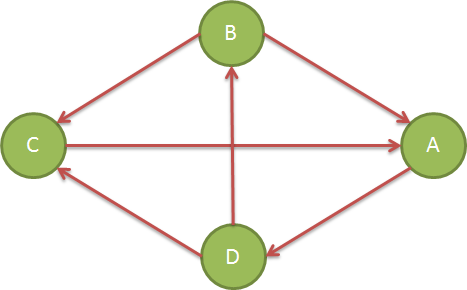
\includegraphics[width=0.65\textwidth]{media/chapter6/pr-example-graph.png}
\caption{Example graph to demonstrate the original Pagerank algorithm.}
\label{fig:pr-graph-example}
\end{figure}

The model introduced by Page and Brin also included a damping factor. Extending the random surfer analogy, this damping factor corresponds to the probability that the surfer stops clicks. At every page the surfer visits, there is a non-zero probability that he will stop surfing. Taking this consideration, the above equation to compute the new pagerank of node A becomes $d(PR(B)/2 + PR(C) + PR(D)/3) = 0.41225$, for d = 0.85. 


\restylealgo{ruled}
\SetAlgoSkip{}
\begin{algorithm}[h!]
\dontprintsemicolon 
\Begin{
  
$R_0$ $\leftarrow$ S  \\
\textbf{loop}: \\
\Indp
  $R_{i+1}$ $\leftarrow$ $AR_i$ \\
  d $\leftarrow$ $||R_i||_1$ - $||R_{i+1}||_1$ \\  
  $R_{i+1}$ $\leftarrow$ $||R_i||_1$ + dE \\
  $\delta$ $\leftarrow$ $||R_{i+1} - R_i||_1$ \\
\Indm
\textbf{while $\delta$ $>$ $\epsilon$}
}
\caption{Original Pagerank Algorithm}
\label{alg:pr-alg}
\end{algorithm}

Mathematically, the pagerank algorithm is expressed as shown in algorithm \ref{alg:pr-alg}. R is a vector over all the nodes in the graph. A is an adjacency matrix where each cell measures is the reciprocal of outgoing edge count. If $u$ and $v$ are two nodes, and there are $N_u$ outgoing edges from $u$ and one of them ends in $v$, then $A(u, v) = 1/N_u$. The expression $||R||_1$ is the L1 or Manhattan norm of a vector $R$, which is computed as $\sum_{\forall i} |R_i|$. The vector $S$ is the initial score assigned to the nodes. On a large scale, pagerank scores are computed using the MapReduce framework \cite{dean2008mapreduce}.

\section{Rank Propagation in Context Networks}

In order to rank candidates for a new given photo, we go by the observation that people participate in similar kinds of types, and spend time with similar groups of people. In other words, the distribution of people in events is not random. By ranking events, we are ordering them by some metric of similarity with respect to the context network containing the new photo. Events encapsulate heterogeneous information. Thus, their similarities must be computed across the different kinds of entities they encapsulate. For example, two event instances of the same class which have no common participating object are less similar to each other than two others which are of the same type and contain same participating objects.

For our application of face tagging, computing similar similarities across time, space, type and object information of events. In order to formalize our rank propagation mechanism, we introduce the concept of a propagation function. A propagation function will transfer score from one event to the other for a specific property of the event. For example, if we can design a propagation algorithm around two functions \texttt{temporal} and \texttt{spatial} propagation, scores will be transferred based only on the temporal and spatial attribute values of the events respectively. We say that the propagation function contributes a \textit{transfer ratio} across a dimension. We follow the same algorithm as the one shown in algorithm \ref{alg:pr-alg} with the following differences: \textbf{First}, the vector $S$ is setup based on the distribution of persons present and the attributes of the events in the new context networks. \textbf{Second}, the matrix $A$ is computed as the L1 norm of a vector over the propagation function transfer score between two events. For two events, $u$ and $w$, and propagation functions $P_t$ and $P_s$ (temporal and spatial propagations), the propagation vector $V$ = $[P_t, P_s]$, and the score transfer vector from $u$ to $w$, $V(u, w)$ = $[P_t(u, w), P_s(u, w)]$ and the value $A(u, w)$ = $||V(u, w)||_1$.

\subsection{Propagation Functions}

In this section we introduce the propagation functions used in our work to rank events for the face tagging application.

\begin{itemize}
\item \textbf{Temporal Propagation}: The temporal propagation function $P_t (u, w)$ propagates a fraction of the score of node $u$ to $w$ proportional to the difference between \texttt{u.duration} and \texttt{v.duration}. The transfer function can be modeled using uniform gaussian or zipf distributions. The advantage with such distributions is to model high transfer of scores who occur nearby in the temporal dimension, and ignoring those which happened too far away. The distribution parameters will be constant and set by the designer.

\item \textbf{Spatial Propagation}: Similar to the temporal propagation function, this takes into consider the spatial attributes of an event while transferring scores.

\item \textbf{Type Propagation}: The class of the event instance is taken into consideration to compare two events. We use the concept of ontological distance to compute the type propagation score transfer. We extend the concept of \texttt{Is-A} distance given in \cite{ranwez2006ontological}. For given a subsumption hierarchy, $a$ is an ancestor of $b$ iff there is a path between $a$ and $b$. The set of concepts having a as ancestor is denoted by $desc(a)$, while its ancestors are denoted as $ansc(a)$. The set of exclusive ancestors (if a node is an ancestor of exactly one of the two nodes) of $a$ and $b$ is denoted by $exAnsc(a, b)$. The subsumption ontological distance is defined as:

$d_{IS}(a, b) = |desc(exAnsc(a, b) \cup desc(a) \cup desc(b) - desc(a) \cap desc(b)|$.

Events also exhibit subevent relationships. Two events could have very common subevents, but might have significant subsumption distance. In this case, we want to reduce this distance. We introduce the subevent distance as the number of common subevents as the number of common descendant in the subevent hierarchy of the ontology. For a node $a$, $subdesc(a)$ is the set of all $a$'s subevents and their transitive descendants.

$d_{SE}(a, b) = |subdesc(a) \cap subdesc(b)|$

Our ontology distance is the sum of subsumption distance and the subevent distance. This number can be normalized with the number of perdurant classes present in the ontology.

$d(a, b) = D_{IS}(a, b) + D_{SE}(a, b)$

\item \textbf{Object Propagation}: If two events have the same set of participating objects, then the score transfered through object propagation is very high. If they have no common objects, then this transfer would be 0. We use Jacquard index to compute this ratio. For two sets of objects $A$ and $B$, the jacquard index is computed as:
\begin{equation}
J(A, B) = \frac{A \cap B}{A \cup B} \nonumber
\end{equation}

\item \textbf{Structural Propagation}: The last propagation function we use is the propagation from an event to its instance subevents. Here we use a function which is similar to the one used in pagerank while computing the transfer from a graph node through an outgoing edge. If event $B$ is a subevent of $A$ (we can use the web graph as an analogy where the subevent edge is an outgoing edge from $A$ to $B$), and $A$ has $n$ subevents, then the propagation ratio from $A$ to $B$ is $1/n$.

\end{itemize}

We could create additional functions which are combinations of these functions. For example, if an event $A$ occurred a long before $B$, and it has common entities, then the object similarity could be weighed based on the spatio-temporal proximity of the two events. In this work, we do not consider such cases.

\section{Experiments}

\begin{figure}[t]
\begin{minipage}[b]{0.5\linewidth}
\centering
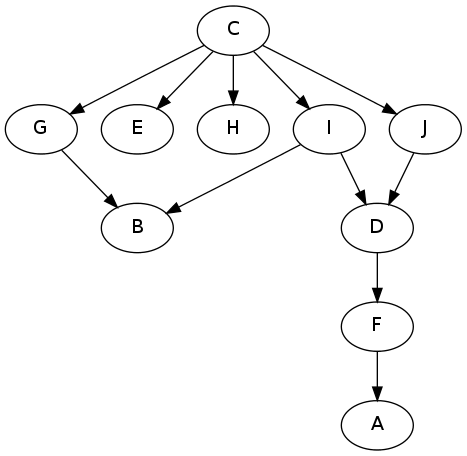
\includegraphics[width=0.7\textwidth]{media/chapter6/sample-ontology.png}
\caption{Example of a subsumption hierarchy created as part of the ontology generation process.}
\label{fig:sample-ontology}
\end{minipage}
\hspace{0.5cm}
\begin{minipage}[b]{0.45\linewidth}

\begin{tabular}{ |c|c|c|c|c|c|c|c|c|c| }
  \hline
  \texttt{A} & \texttt{B} & \texttt{C} & \texttt{D} & \texttt{E} & \texttt{F} & \texttt{G} & \texttt{H} & \texttt{I} & \texttt{J} \\
  \hline
    0  &  6  &  9  &  2  &  7  &  1  &  7  &  7  &  5  &  5 \\
    6  &  0  &  9  &  6  &  7  &  6  &  5  &  7  &  5  &  7 \\
    9  &  9  &  0  &  7  &  9  &  8  &  8  &  9  &  5  &  6 \\
    2  &  6  &  7  &  0  &  7  &  1  &  7  &  7  &  3  &  3 \\
    7  &  7  &  9  &  7  &  0  &  7  &  3  &  2  &  6  &  5 \\
    1  &  6  &  8  &  1  &  7  &  0  &  7  &  7  &  4  &  4 \\
    7  &  5  &  8  &  7  &  3  &  7  &  0  &  3  &  5  &  6 \\
    7  &  7  &  9  &  7  &  2  &  7  &  3  &  0  &  6  &  5 \\
    5  &  5  &  5  &  3  &  6  &  4  &  5  &  6  &  0  &  3 \\
    5  &  7  &  6  &  3  &  5  &  4  &  6  &  5  &  3  &  0 \\
  \hline
\end{tabular}
\caption{The \texttt{is-A} distance between classes in figure \ref{fig:sample-ontology}.}
\label{tbl:semantic-distance}
\end{minipage}
\end{figure}

We investigate the convergence behavior of our propagation algorithm. To simulate this experiment, we use the generative model described in section \ref{section:generative_models}. We generate an ontology using the following steps: A random number of entities are chosen, and a subsumption hierarchy is created (similar to the one shown in \ref{fig:sample-ontology}) a fraction of the events are assigned a subevent hierarchy, which uses the step described in section \ref{section:generative_models}. For this experiment we restrict the depth of the subevent hierarchy to be 2, and each event class has atmost 3 subevents. Events are instantiated randomly. We generate 1000 events for this experiment. It must be noted that this is a fairly large number as we are propagating scores for each event to all the others one due to temporal and spatial propagations. Thus, for 1000 events, we expect a million propagations per iteration. We use a linear distribution for spatial and temporal propagation functions. For the temporal function, this means that the propagation decreases linearly until 5\% of the total timespan of the events, at which point it becomes 0. Similarly spatial propagation decreases 10\% of the maximum distance between two event instances in the dataset (these percentages were arbitrarily chosen).

\begin{figure}[h!]
\centering
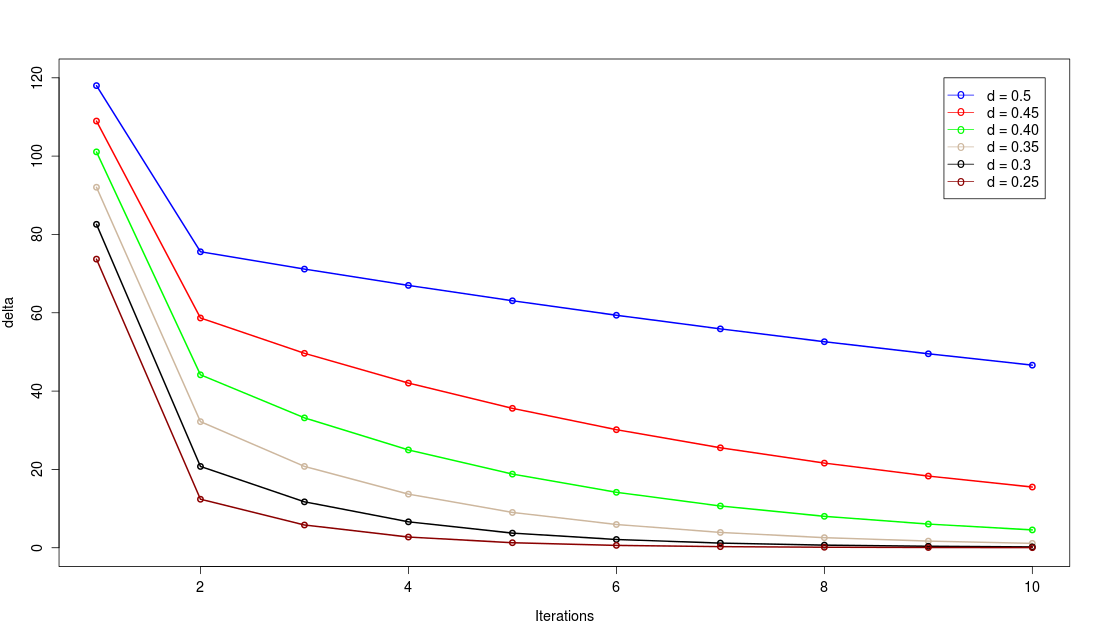
\includegraphics[width=0.85\textwidth]{media/chapter6/convergences.png}
\caption{Rate of convergence of the propagation algorithm for varying values of $d$.}
\label{fig:convergences}
\end{figure}

Figure \ref{fig:convergences} plots the L1 norm in the rank vector for different values of the decay factor per iteration. For a higher value of the decay factor, $d$, we see a faster convergence rate. It must be noted that for this convergence is achieved within a few iterations. We also plot the rate of convergence for datasets with different number of instances. In figure \ref{fig:convergences-inreasing-nodes}, we plot the decreasing value of $\delta$ on a log scale for two datasets, one containing 1000 nodes, and the other with 1500 nodes. The plot shows the increasing number of iterations for larger datasets to converge to the same value.

\begin{figure}[h]
\centering
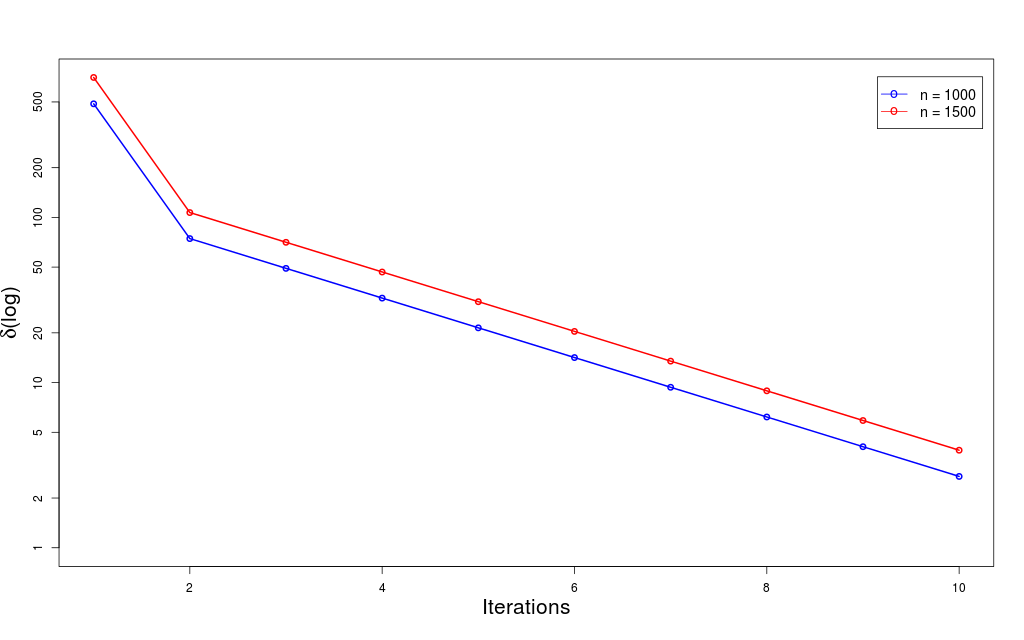
\includegraphics[width=0.85\textwidth]{media/chapter6/convergence-with-node-change.png}
\caption{Rate of convergence with increasing number of instances, for $d$ = 0.85.}
\label{fig:convergences-inreasing-nodes}
\end{figure}

